\chapter{Kapiel 1}

\begin{enumerate}[label=\arabic*.]
    \item \textbf{Wieso spricht man im Kontext von Prozessen von einer `Illusion der Parallelität'?} \newline
          \textit{Antwort:} Weil immer nur ein Prozess gleichzeitig laufen kann, jedoch wechseln Prozesse sich
          so schnell ab, dass es für einem Menschen so vorkommt, als würden diese Paralell laufen.

    \item \textbf{Wie erhält der Scheduler selbst die Prozessorzeit?} \newline
          \textit{Antwort:} Nach jedem Interrupt wird der Scheduler aufgerufen. Dieser entscheidet, wie fortgefahren
          werden soll.

    \item \textbf{Nennen Sie 3 elementare Betriebsmittel und ihren Nutzen.} \newline
          \textit{Antwort:} \begin{itemize}
              \item \textit{CPU:} Führt Arithmetische und Boolische berechnungen durch.
              \item \textit{Speicher:} Dort werden Daten zur späteren Nutzung abgelegt.
              \item \textit{Kommunikationsverbindungen:} Ist die Physische verbindung zwischen den einzelnen
                    Hardwarekomponenten eines Computers. \newline (Z.B.: der Datenbus.)
              \item \textit{\texttt{I/O}-Geräte:} Dienen zur Ein-/ und Ausgabe von Informationen.
          \end{itemize}

    \item \textbf{Erklären Sie was ein Betriebssystem ist nach dem Top-Down (Bottom-Up) Prinzip.} \newline
          \textit{Antwort:} Das Betriebssystem soll die `hässliche' Hardware verbergen. Der Endnutzer soll nicht
          mitbekommen, welche Unangenehmen Aufgaben wie Unterbrechungen, \texttt{I/O}-Zugriffe
          etc.\ durchgeführt werden.

    \item \textbf{Nennen Sie sämtliche Betriebssystemfamilien, die Sie in der Vorlesung kennengelernt
              haben und beschreiben Sie kurz wie / wo sie eingesetzt werden.} \newline
          \textit{Antwort:} \begin{itemize}
              \item \textit{Großrechner}: In industriellen Einrichtungen, wo sehr viel Leistung erforderlich ist
                    um beispielsweise viele, sehr \texttt{I/O}-Lastige Prozesse durchzuführen.
              \item \textit{Server}: Sollen viele Nutzer gleichzeitig über das Netzwerk bedienen.
              \item \textit{Multiprozessorsysteme}: Computer mit mehreren Prozessoren.\newline Können überall eingesetzt werden.
              \item \textit{PCs}: Personalisierbare Computer für z.B. Privatpersonen.
              \item \textit{Handheld Computer}: Computer, welche `in der hand' liegen und Portabel mitgenommen
                    werden können.
              \item \textit{Eingebettete Systeme}: Simple Computer welche meist eine oder wenige Aufgaben erfüllen wie
                    z.B. die Steuerung anderer Geräte.
              \item \textit{Sensorknoten}: Führen kontinuierliche Messungen durch und übertragen diese Daten meist
                    an andere Systeme.
              \item \textit{Echtzeitsysteme}: Müssen Aufgaben in einer fest vorgelegten Zeit durchführen.
              \item \textit{Smartcards}: Sollten sehr klein sein und führen idr.\ nur wenige Funktionen
                    durch, z.B. Bezahlen.
          \end{itemize}

    \item \textbf{Was ist der Unterschied zwischen weichen und harten Echtzeitsystemen?} \newline
          \textit{Antwort:} \begin{itemize}
              \item \textit{Harte Echtzeitsysteme:} Bei Harten Echtzeitsystemen ist eine zu späte
                    berechnung der Daten ein Fehler, welcher z.B. zu Abbruch des Systemes führen kann.
                    Das Betriebssystem darf die Laufzeit des Prozesses nicht verlangsamen.
              \item \textit{Weiche Echtzeitsysteme:} Zu späte lieferung von Daten ist nicht erwünscht,
                    führt aber nicht zu einem Fehler.
          \end{itemize}

    \item \textbf{Was ist der Unterschied zwischen einem Prozess und einem Programm?} \newline
          \textit{Antwort:} Ein Prozess ist ein Programm in Ausführung.

    \item \textbf{Welche 4 elementaren Dinge gehören zu einem Prozess und was ist deren Funktionen?} \newline
          \textit{Antwort:} \begin{itemize}
              \item \textit{Das ausführbare Programm:} gibt vor, wie sich der Prozess verhalten soll.
              \item \textit{Programmdaten:} speichert die Daten des Programms
              \item \textit{Stack-Bereich:} Gibt den Bereich des Stacks vor
              \item \textit{CPU-Register einschließlich Programmzähler und Stackpointer:} Gibt beispielsweise
                    den ProgrammCounter vor.
          \end{itemize}

    \item \textbf{Welche Kontextarten in Bezug auf Prozessen kennen Sie?} \newline
          \textit{Antwort:} Pid (ProzessID), Gid (GroupID), Uid (UserID)

    \item \textbf{Nennen Sie mindestens 3 Aufgaben, die man mit Systemaufrufen erledigen kann.} \newline
          \textit{Antwort:} \begin{itemize}
              \item Timer
              \item Prozess erzeugen
              \item Datei Öffnen
              \item Up bzw Down operation bei Semaphoren
          \end{itemize}

    \item \textbf{Wie läuft ein Systemaufruf / System Call ab? Sie können auch eine Skizze anfertigen.} \newline
          \textit{Antwort:} Ein Benutzerprogramm ruft die Bibliotheksprozdur auf. Diese bereitet die Daten vor und
          sendet eine Trap an das Betriebssystem. Das Betriebssystem führt den Systemaufruf durch und gibt die Daten
          zurück an die Bibliotheksprozdur. Diese bereitet dann die Daten auf und gibt sie zurück an den Benutzerprogramm.

          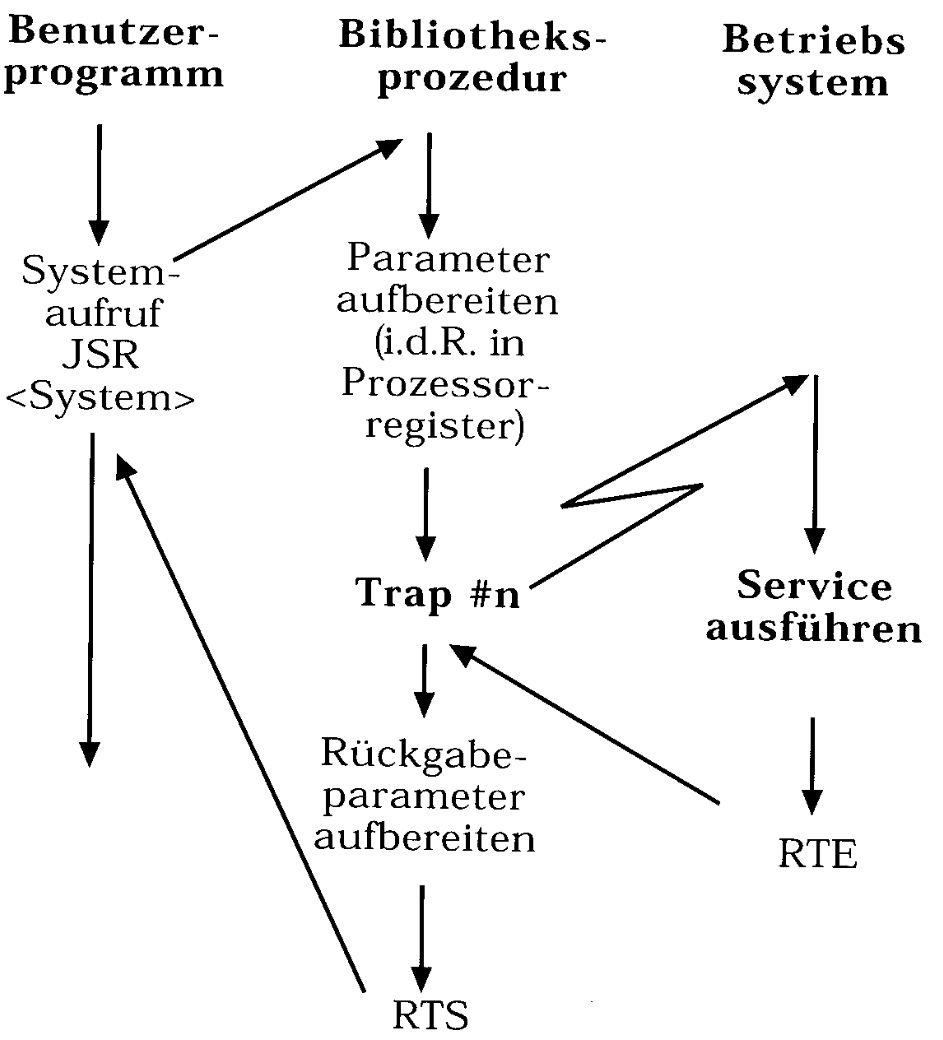
\includegraphics[width=\textwidth]{assets/systemaufruf.png}

    \item \textbf{Erläutern Sie pid, uid und gid.} \newline
          \textit{Antwort:} \begin{itemize}
              \item \textit{pid:} Die ProzessID.\ Hierrüber kann der Prozess gesteuert und beispielsweise beendet werden.
              \item \textit{uid:} Die UserID.\ Jeder Nutzer erhält eine eigene, einzigartige ID mit welcher die Benutzer
                    voneinander unterschieden werden können. Hierrüber kann ein Prozess beispielsweise einem User zugewiesen werden.
              \item \textit{gid:} Die GruppenID.\ Mehrere Nutzer können in einer Gruppe gruppiert werden, um beispielsweise
                    einem Prozess mehreren Nutzern zuzuweisen.
          \end{itemize}

    \item \textbf{Was versteht man unter einem Hardware-Interrupt?} \newline
          \textit{Antwort:} Ein Interrupt, der von der Hardware gesendet wird. Beispielswesie ein Timer-Interrupt.

    \item \textbf{Erklären Sie den Begriff Swapping.} \newline
          \textit{Antwort:} Beim Swapping werden Zugehörige Daten komplett in den Haupspeicher geladen. Alle Daten,
          welchen zu einem Prozess gehören, sind im Hauptspeicher.

    \item \textbf{Was ist der Scheduler und was sind seine Aufgaben?} \newline
          \textit{Antwort:} Der Scheduler gibt vor, welche Prozesse wann laufen dürfen. Er entscheidet, welcher
          Prozess als nächstes laufen darf.

    \item \textbf{Was bedeutet Relokation?} \newline
          \textit{Antwort:} Bei der Relokation werden Adressen mit einem bestimmten Offset zu den phsysischen Adressen
          adressiert. Virtuelle Adressen werden in physische Adressen umgerechnet.

    \item \textbf{Erklären Sie den Begriff Paging?} \newline
          \textit{Antwort:} Beim Paging wird der Speicher in virtuelle Seiten mit fester Größe aufgeteilt.
          Diese Seiten können in beliebiger Reihenfolge auf den Hauptspeicher zugewiesen und, falls sie nicht
          benötigt werden, in den Hintergrundspeicher geladen werden.

    \item \textbf{Wo liegen die Unterschiede zwischen virtueller und realer Adressierung?} \newline
          \textit{Antwort:} Bei realer adressierung wird direkt auf den Hauptspeicher zugegriffen, bei virtueller
          Adressierung existieren die Adressen nicht reale. Virtuelle Adressierung besitzt meist viel mehr Speicher
          als reale Adressierung.

    \item \textbf{Was ist eine Shell?} \newline
          \textit{Antwort:} Die Shell ist eine Commandozeile und dient zur Kommunikation mit dem Betriebssystem.
          Sie nimmt Benutzerbefehle entgegen und bringt diese zur Ausführung.

    \item \textbf{Nennen Sie 6 Betriebssystemstrukturen und erläutern Sie \newline kurz ihre Funktion.} \newline
          \textit{Antwort:} \begin{itemize}
              \item \textit{Monolithische Systeme:} Das Betriebssystem ist der einzige Prozess im Kernmodus.
              \item \textit{Geschichtete Systeme:} Das Betriebssystem ist in Schichten aufgeteilt. Jede Ebene ruft
                    die nächst tiefere auf.
              \item \textit{Mikrokerne:} Das Betriebssystem ist in mehrere Module aufgeteilt. Das Betriebssystem wird
                    als einziges Modul im Kernmodus ausgeführt.
              \item \textit{Client-Server-Modell:} Der Client fragt Dienste von den Server an. Der Server stellt
                    für den Client Dienste zur verfügung.
              \item \textit{Virtuelle Maschinen:} Ein Betriebssystem, welches auf einem Gastgeberbetriebssystem
                    virtuell läuft.
              \item \textit{Exokerne:} Jeder nutzer bekommt einen Teil der Betriebsmittel zugewiesen. Es werden
                    mehrere voneinander unabhängige Virtuelle Maschinen bereit gestellt.
          \end{itemize}

    \item \textbf{Nennen Sie 3 Einsatzgebiete für virtuelle Maschinen.} \newline
          \textit{Antwort:} \begin{itemize}
              \item Isolation von Benutzern
              \item Test von neuen Geräten
              \item Übergang zu neuer Anlage
              \item Betriebssystemtest
              \item FTP-Server
              \item Mailserver
              \item Webserver
          \end{itemize}

    \item \textbf{Erklären Sie den Typ 1 - Hypervisor. (Oder auch Typ 2 - Hypervisor)} \newline
          \textit{Antwort:} \begin{itemize}
              \item \textit{Typ 1 - Hypervisor:} Die Virtuelle Maschine läuft in einem Prozess auf dem
                    Gastgeberbetriebssystem. Anfragen an Systemressourcen müssen erst an das Gastgeberbetriebssystem
                    gestellt werden. Diese werden dann von dem Gastgeberbetriebssystem bereit gestellt.
              \item \textit{Typ 2 - Hypervisor:} Die einzige Aufgabe des Betriebssystems ist es,
                    Virtuelle maschinen bereit zu stellen. Anfragen an Systemressourcen können unmittelbar 
                    bereitgestellt werden.
          \end{itemize}

    \item \textbf{Was versteht man unter einem Exokern?} \newline
          \textit{Antwort:} Jeder nutzer bekommt einen Teil der Betriebsmittel zugewiesen. Es werden
                    mehrere voneinander unabhängige Virtuelle Maschinen bereit gestellt. Der Exokern 
                    sorgt dafür, dass alle Prozesse voneinander abgekapselt sind und keine Virtuelle 
                    Maschine auf die Systemressourcen einer anderen zugreifen kann.

\end{enumerate}